\begin{figure}
\centering
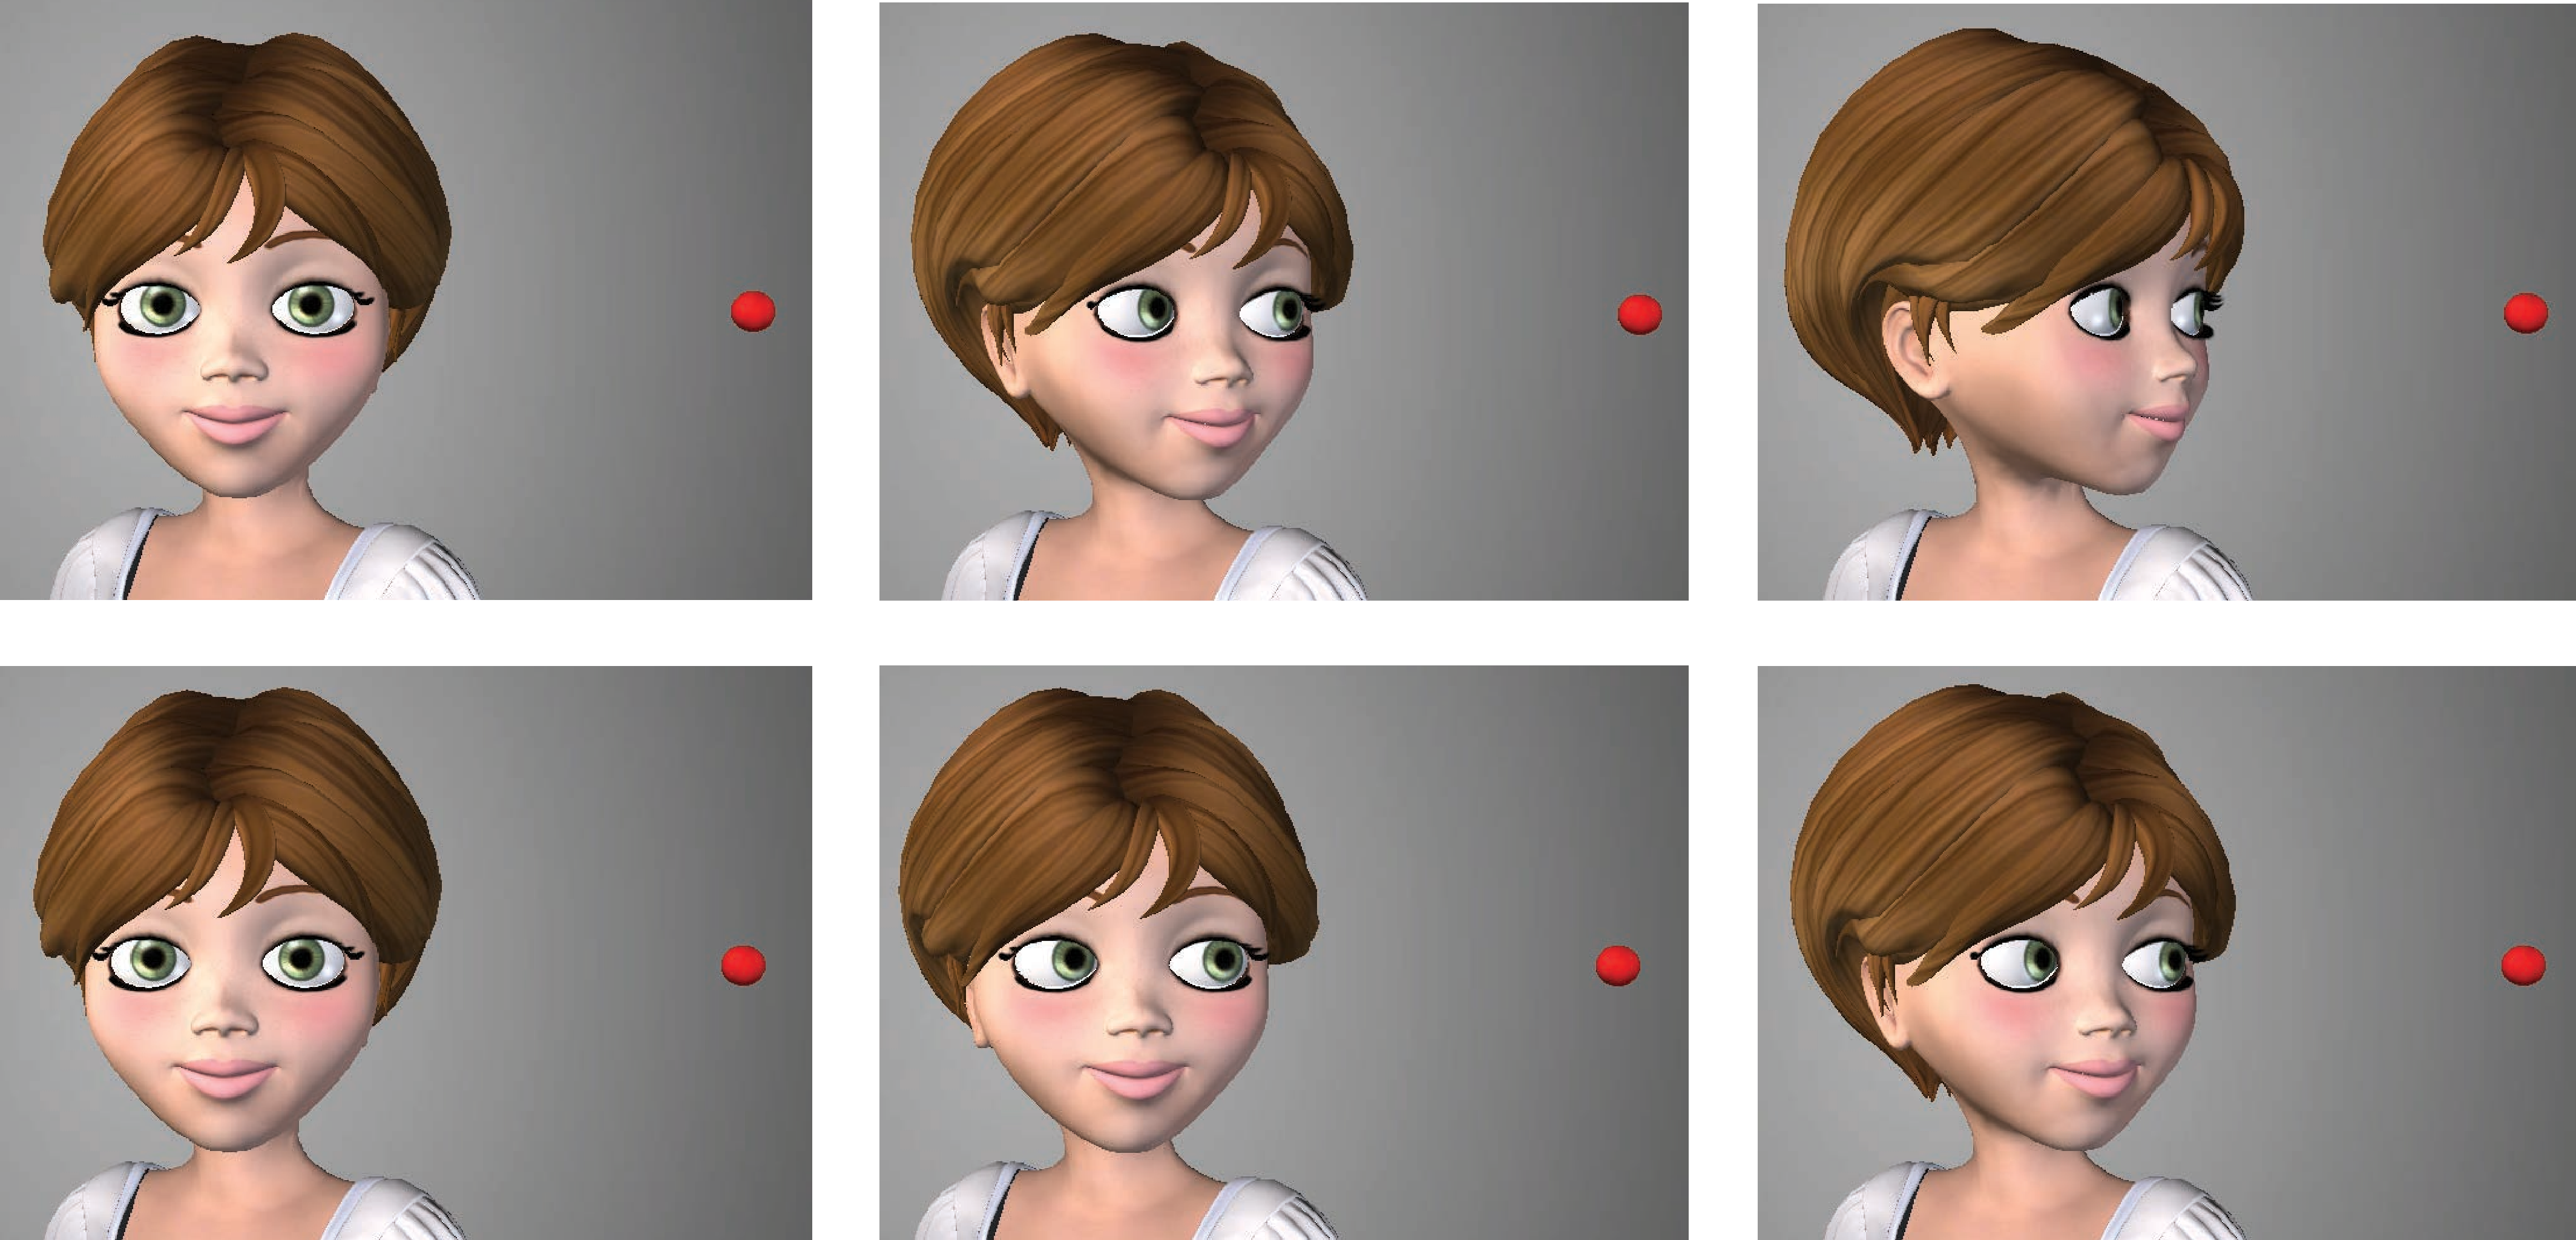
\includegraphics[width=0.9\textwidth]{stylizedgaze/Figures/PerformativeGazeExample-small.pdf}
\caption{A performative gaze shift. Top: The character fully aligns its gaze with the red sphere. Bottom: The character partially aligns its gaze with the target ($\alpha_E = 0.7$) but still appears to be gazing at it, because it has achieved screen-space alignment.}
\label{fig:PerformativeGazeExample}
\end{figure}

\begin{figure}
\centering
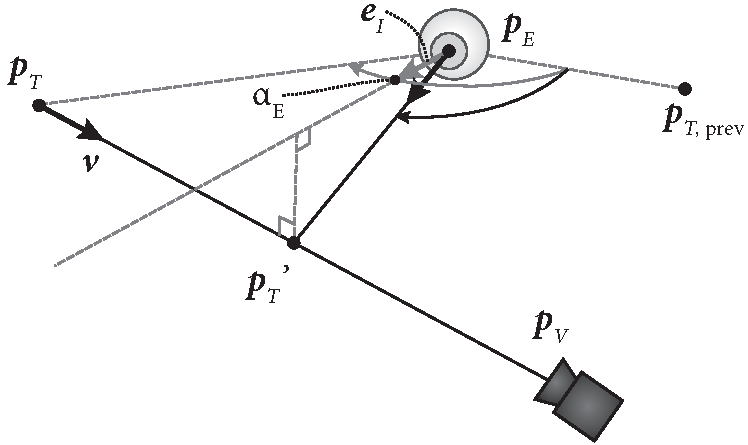
\includegraphics[width=0.75\textwidth]{stylizedgaze/Figures/EyeAlignment.pdf}
\caption{The calculation of the effective gaze target position in a performative gaze shift.}
\label{fig:EyeAlignment}
\end{figure}

While humans use gaze to seek information in the environment, in acting and cartoon animation, the primary purpose of gaze is to communicate ideas and create engagement with an audience. These goals can be achieved by performing partial gaze shifts in the general direction of the object of interest in order to convey the idea that the character is attending to the object without actually aligning its eyes with it. This performative behavior allows the character to retain partial alignment with the audience, enabling them to better see what the character is doing and making the performance more immediate and engaging. The notion that viewers prefer it when a virtual character or real person faces them more is strongly supported by research, e.g.,~\citep{beebe1976effects,andrist2012designing}.

We introduce a motion adaptation method for gaze shifts that allows the synthesis of performative gaze shifts. The method exposes an eye alignment parameter, $\alpha_E$, which allows the animator to specify the desired amount of alignment with the target. Setting $\alpha_E = 1$ causes the eyes to fully align with the target.
% NOTE: More detailed explanation of how the parameter can be tweaked -- Tomislav
With parameter values lower than $1$, the character will gaze toward a point directly between the gaze target and the viewer, which we call the \textit{effective gaze target}. In order to convince the viewer that the character is gazing toward the real target, the two targets must line up in the screen space, as illustrated in Figure~\ref{fig:PerformativeGazeExample}.

Figure~\ref{fig:EyeAlignment} illustrates how the specified eye alignment is achieved. We compute the intermediate rotation of each eye using $\mathbf{q}_I = slerp (\mathbf{q}_S, \mathbf{q}_T, \alpha_E )$, where $\mathbf{q}_S$ and $\mathbf{q}_T$ are the eye orientations in the source and target pose, respectively. At this orientation, the eye's gaze direction is given by the ray $\mathbf{e}_I$. The view direction ray, $\mathbf{v}$, points from the target position $\mathbf{p}_T$ to the viewer. Effective gaze target position, $\mathbf{p}_T'$, is the point along the ray $\mathbf{v}$ that is the closest to the ray $\mathbf{e_I}$.

Similar to the target pose adaptation techniques described in Section~\ref{sec:StylizedGazeTargetPoseAdaptation}, partial eye alignment is applied in a view-dependent manner. At low target viewing angles, $\phi_T$, the method enforces full eye alignment to prevent the viewer from noticing that the character is not actually gazing at them by automatically adjusting it using the viewing cone parameter, $p_{\phi}$, as follows:
%
\begin{equation}
\alpha_E' = 1 - p_{\phi} + \alpha_E p_{\phi}.
\end{equation} 